\documentclass[10pt,a4paper]{AMdocument}
\usepackage[utf8]{inputenc}
\usepackage{caption}

%-> bibliography settings
\usepackage{AMbiblio}
\addbibresource{references.bib}

%-> titlepage settings
\title{Investigation of energy conserving Hyper Reduction Techniques for nonlinear FE}
\subtitle{Master of Science project}
\author{Johannes Rutzmoser}
\contactphone{+49-89-289-15202}
\contactemail{johannes.rutzmoser@tum.de}
\AMsetTitlepage{contact}

%-> other settings
\AMsetColor{titles=TUMDarkBlue,caption label=TUMDarkBlue,cite=black,abstract=TUMDarkBlue}
\AMsetFont{theme=tumhelvetica,section title size=\normalsize}
\AMsetLayout{page geometry={top=0.8cm,left=1.7cm,right=1.7cm,bottom=0.8cm},page style=empty}


\begin{document}
\maketitle

\begin{abstract}
   The M.Sc. project aims at studying energy conserving Hyper Reduction Techniques to reduce the assembly costs for geometrically and material nonlinear Finite Element models. After a literature review, the student should implement the Energy Conserving Mesh Sampling and Weighting (ECSW) Method in the Nonlinear Finite Element Code AMfe. The method requires a computationally expensive training simulation of the unreduced system. This issue shall be tackled within this the thesis. 
\end{abstract}

\begin{figure}[h]
   \centering
   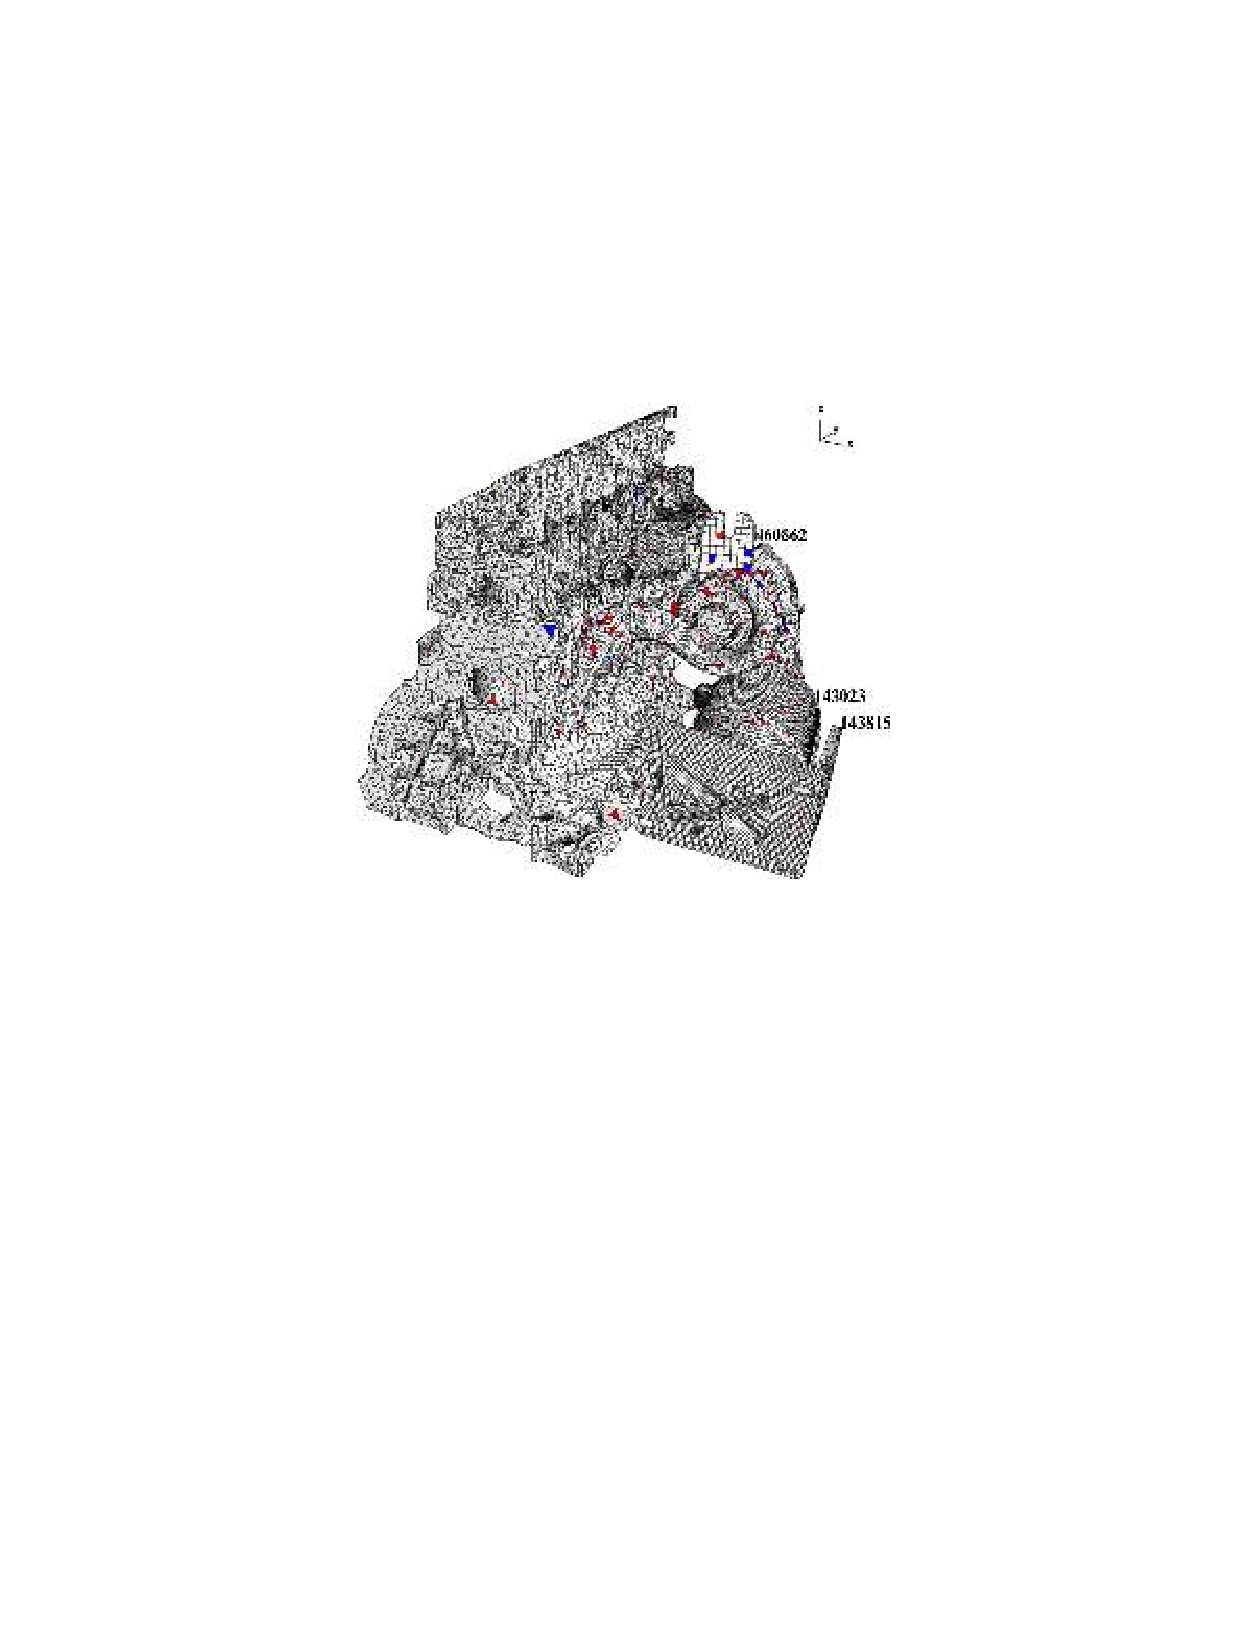
\includegraphics[width=0.4\linewidth]{Bilder/farhat_engine.pdf}
   \caption{Full car engine with reduced mesh (red) for using ECSW, taken from \cite{farhat2015structure}}
\end{figure}

\paragraph{Introduction}
In the realm of nonlinear Model Order Reduction for structural mechanics, two main tasks have to be solved: 
First, the choice of a proper reduction basis suitable for the problem resulting in a system with less degrees of freedom. Secondly, the reduction of the assembly process of the nonlinear force vector and the tangent stiffness matrix, by generating a reduced mesh. This task is called Hyper Reduction. 

Whereas most hyper reduction techniques aim at the approximation of the high dimensional nonlinear vector, a recent development called Energy Conserving Mesh Sampling and Weighting (ECSW) aims at the approximation of the virtual work, which results in a much more efficient evaluation of the nonlinear force while maintaining intrinsic properties of the mechanical system. 

As the ECSW method is fairly young, many questions regarding technical details are still open. Furthermore, the method as proposed by \textsc{Farhat} \cite{farhat2015structure} requires very expensive training simulations, which are often not possible without huge computer grids.


\paragraph{Tasks}
1) Conduct a literature review regarding Hyper Reduction techniques with a special focus on methods, which conserve the mechanical properties like symmetry, stability and an underlying variational formulation. 
2) Implement the ECSW method in the nonlinear Finite Element framework AMfe developed at the Chair of Applied Mechanics at Technische Universität München (TUM). 
3) Investigate the ECSW regarding technical aspects like parameters, models of different size and complexity, and error measures by means of numerical experiments. 
4) Further develop the ECSW method by using heuristically generated displacement fields substituting the unreduced training simulation. The Instutite of Applied Mechanics has some promising pre-studies on that topic. 
5) Present the results in a report and a peer-reviewed journal paper.

\paragraph{Requirements}
The student should have good experience and knowledge of the Finite Element Method, especially in nonlinear formulations. Programming skills with the Python language are recommended.

\printbibliography
\end{document}